\documentclass[a4paper]{article}

\usepackage[ngerman]{babel}
\usepackage[utf8]{inputenc}
\usepackage{enumitem}
\usepackage{amsmath}
\usepackage{array}
\usepackage{graphicx}
\newcolumntype{L}{>{$}c<{$}}


\title{Grundlagen der Rechnerarchitektur\\ Übungsblatt 6\\Gruppe 121\\}
\author{Jonas Otto\and Dominik Authaler}

\date{\today}

\begin{document}

\maketitle

\section*{Aufgabe 1}
\begin{enumerate}[label=\alph*)]
	\item Wahrheitstafel:
	\begin{figure}[h!]
		\centering
		\begin{tabular}{|c|c|c|}
			\hline
			Tag & Tag - 1 binär ($x_3x_2x_1x_0$) & Angeschaltete Äste \\
			\hline
			1 & 0000 & 1, 2, 3, 4, 5, 6, 7\\
			2 & 0001 & 2, 4, 6\\
			3 & 0010 & 2, 4, 6\\
			4 & 0011 & 1, 2, 4, 6\\
			5 & 0100 & 2, 4, 6\\
			6 & 0101 & 1, 2, 3, 4, 5, 6\\
			7 & 0110 & 1, 2, 3, 4, 5, 6\\
			8 & 0111 & 1, 2, 3, 4, 5, 6, 7\\
			9 & 1000 & 1, 3, 5\\
			10 & 1001 & 1, 2 3, 4, 5, 6\\
			11 & 1010 & 1, 3, 4, 5, 6\\
			12 & 1011 & 1, 3, 5\\
			13 & 1100 & 1, 3, 5\\
			14 & 1101 & 1, 2, 3, 4, 5, 6\\
			15 & 1110 & 1, 3, 5, 7\\
			16 & 1111 & 1, 2, 3, 5\\
			\hline
		\end{tabular}
		\caption{Wahrheitstabelle zur Ansteuerung der Segmente}
	\end{figure}

	\item Kanonische Normalformen:
	\begin{equation*}
	\begin{aligned}
		f_{1, DKNF} = &\overline{x_0 x_1 x_2 x_3} + x_0 x_1\overline{x_2 x_3} + x_0 \overline{x_1} x_2 \overline{x_3} + \overline{x_0} x_1 x_2 \overline{x_3} + x_0 x_1 x_2 \overline{x_3} + \overline{x_0 x_1 x_2} x_3 \\
		&+ x_0 \overline{x_1 x_2} x_3 + \overline{x_0} x_1 \overline{x_2} x_3 + x_0 x_1 \overline{x_2} x_3 + \overline{x_0 x_1} x_2 x_3 + x_0 \overline{x_1} x_2 x_3 + \overline{x_0}x_1 x_2 x_3 + x_0 x_1 x_2 x_3
	\end{aligned}
	\end{equation*}
	
	\begin{equation*}
	\begin{aligned}
		f_{2, KKNF} = &(x_0 + x_1 + x_2 + \overline{x_3}) \cdot (x_0 + \overline{x_1} + x_2 + \overline{x_3}) \cdot (\overline{x_0} + \overline{x_1} + x_2 + \overline{x_3})\\ &\cdot (x_0 + x_1 + \overline{x_2} + \overline{x_3}) \cdot (x_0 + \overline{x_1} + \overline{x_2} + \overline{x_3})
	\end{aligned}
	\end{equation*}
	
	\clearpage
	\item Algebraische Minimierung:
	%\begin{equation*}
	%\begin{aligned}
	%	f_{1, DNF} &= f_{1, DKNF} \\ &= \overline{x_0 x_1 x_2 x_3} + x_0 x_1\overline{x_2 x_3} + x_0 \overline{x_1} x_2 \overline{x_3} + \overline{x_0} x_1 x_2 \overline{x_3} + x_0 x_1 x_2 \overline{x_3} + \overline{x_0 x_1 x_2} x_3 
	%	+ x_0 \overline{x_1 x_2} x_3 \\ &+ \overline{x_0} x_1 \overline{x_2} x_3 + x_0 x_1 \overline{x_2} x_3 + \overline{x_0 x_1} x_2 x_3 + x_0 \overline{x_1} x_2 x_3 + \overline{x_0}x_1 x_2 x_3 + x_0 x_1 x_2 x_3 \\
	%	&\stackrel{P4}{=} \overline{x_0 x_1 x_2} \cdot (\overline{x_3} + x_3) + x_0x_1x_2 \cdot (\overline{x_3} + x_3) + \overline{
	%\end{aligned}
	%\end{equation*}
	
	\item Karnaugh-Veitch:
	\begin{enumerate}[label=\roman*)]
		\item minimale disjunkitve Normalform $f_{3, KV, DNF}$ für Segment 3:
		
		\begin{figure}[h]
			\begin{center}
				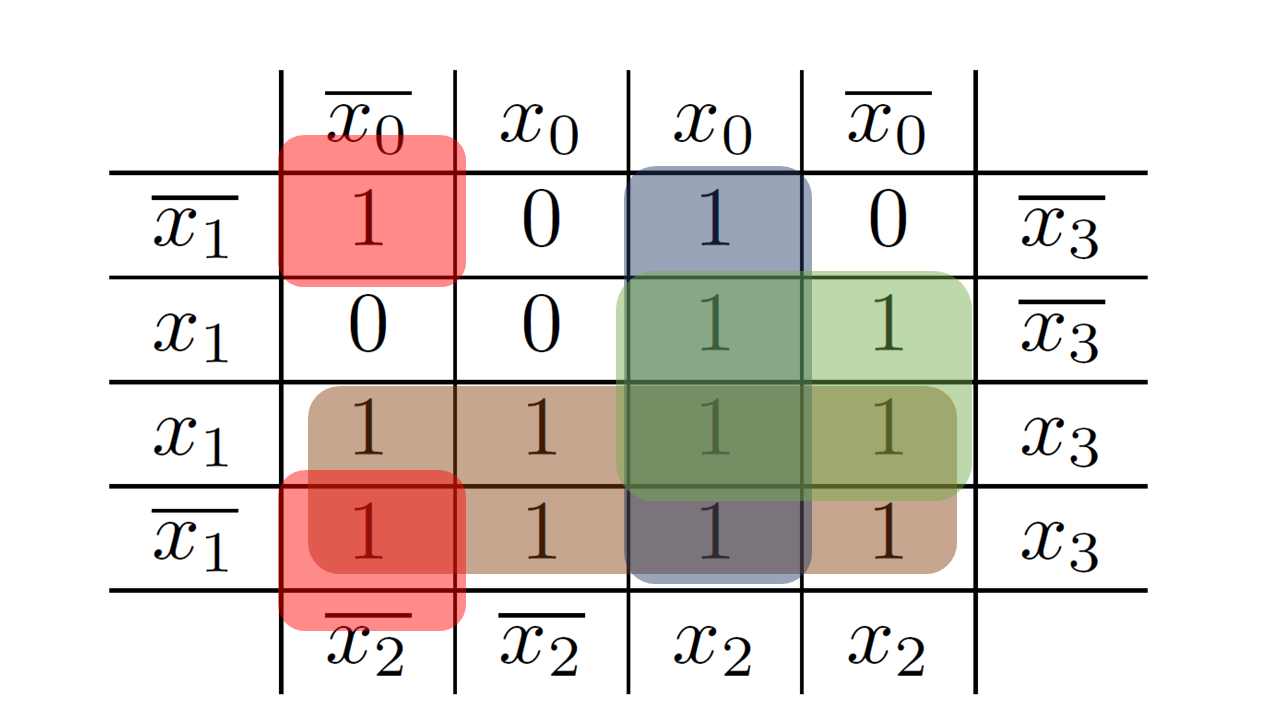
\includegraphics[scale=0.25]{KV-Segment-3.png}
			\end{center}
			\caption{KV-Diagramm für Segment 3}
		\end{figure}
	
		\begin{equation}
			f_{3, KV, DNF} = x_3 + x_1x_2 + x_0x_2 + \overline{x_0 x_1 x_2}
		\end{equation}
		
		
		\item minimale konjunktive Normalform $f_{4, KV, KNF}$ für Segment 4:
		\begin{figure}[h]
			\begin{center}
				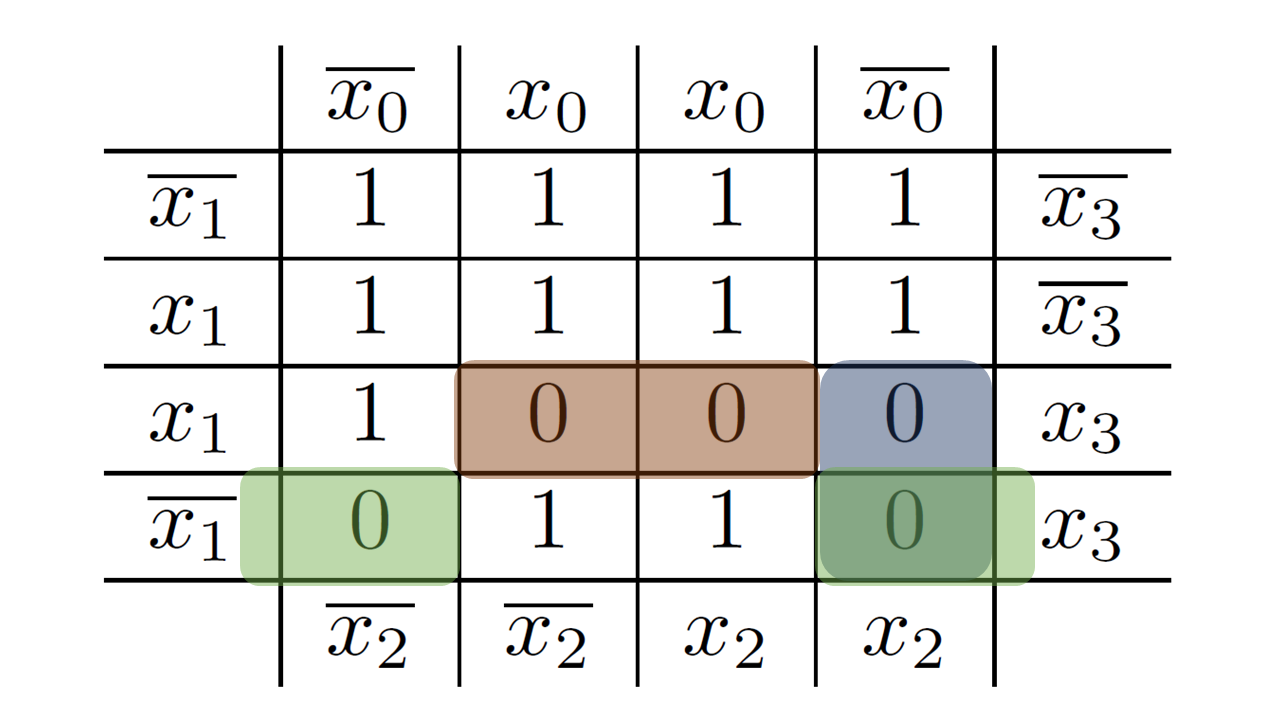
\includegraphics[scale=0.25]{KV-Segment-4.png}
			\end{center}
			\caption{KV-Diagramm für Segment 4}
		\end{figure}
	
		\begin{equation}
			f_{3, KV, DNF} = (x_0 + \overline{x_2} + \overline{x_3}) \cdot (\overline{x_0} + \overline{x_1} + \overline{x_3}) \cdot (x_0 + x_1 + \overline{x_3})
		\end{equation}
	\end{enumerate}
\end{enumerate}

\end{document}
	
